\documentclass[11pt,a4paper]{article}

% ── Fonts & encoding ──────────────────────────────────────
\usepackage{lmodern}
\usepackage[T1]{fontenc}
\usepackage[utf8]{inputenc}

% ── Layout ────────────────────────────────────────────────
\usepackage[margin=28mm]{geometry}
\usepackage{microtype}
\usepackage{parskip}

% ── Math ──────────────────────────────────────────────────
\usepackage{amsmath,amssymb}

% ── Tables ────────────────────────────────────────────────
\usepackage{booktabs}
\usepackage{array}

% ── Colors & headers ──────────────────────────────────────
\usepackage[dvipsnames]{xcolor}
\usepackage{colortbl}
\usepackage{fancyhdr}
\usepackage{titlesec}

% ── Graphics ──────────────────────────────────────────────
\usepackage{graphicx}

% ── Links ─────────────────────────────────────────────────
\usepackage[colorlinks=true,linkcolor=NavyBlue,citecolor=NavyBlue,urlcolor=NavyBlue]{hyperref}

% ── Lists ─────────────────────────────────────────────────
\usepackage[shortlabels]{enumitem}
\setlist{nosep,leftmargin=1.5em}

% ── Section style ─────────────────────────────────────────
\titleformat{\section}{\large\bfseries\color{NavyBlue}}{\thesection}{0.8em}{}
\titleformat{\subsection}{\normalsize\bfseries\color{NavyBlue!80}}{\thesubsection}{0.6em}{}

% ── Footer ────────────────────────────────────────────────
\pagestyle{fancy}
\fancyhf{}
\renewcommand{\headrulewidth}{0pt}
\fancyfoot[L]{\footnotesize Magnusson (2026) -- 10.6084/m9.figshare.32037990}
\fancyfoot[R]{\footnotesize \thepage}

% ── Macros ────────────────────────────────────────────────
\newcommand{\lcdm}{$\Lambda$CDM}
\newcommand{\seff}{$\Sigma_{\mathrm{eff}}$}

\begin{document}

% ══════════════════════════════════════════════════════════
%  TITLE
% ══════════════════════════════════════════════════════════

\begin{center}
{\LARGE\bfseries EFC Perturbation Sector:\\[4pt]
Constraint-Driven Gravitational Slip\\[4pt]
and a Testable Lensing Crossover}

\vspace{10pt}
{\large Morten Magnusson}\\[2pt]
{\small Energy-Flow Cosmology Initiative}\\[2pt]
{\small \href{https://orcid.org/0009-0002-4860-5095}{ORCID: 0009-0002-4860-5095}}

\vspace{8pt}
{\small DOI: \href{https://doi.org/10.6084/m9.figshare.32037990}{10.6084/m9.figshare.32037990}}\\[4pt]
{\small April 2026 --- v1.0}
\end{center}

\vspace{6pt}

% ══════════════════════════════════════════════════════════
%  ABSTRACT
% ══════════════════════════════════════════════════════════

\begin{quote}\small
\textbf{Abstract.}
We derive the complete $(\mu,\Sigma,\eta)$ perturbation system from the
EFC relativistic action and test it against current cosmological data.
The Lagrange-multiplier flow constraint generates anisotropic stress
absent in standard Horndeski theories, enabling a regime where $\mu < 1$
and $\Sigma \geq 1$, whose observable imprint is a redshift-dependent
lensing crossover.
We prove that standard quasi-static Horndeski with $\alpha_T = 0$
\emph{cannot} produce this signature.
Current growth-rate data show no preference for the EFC extension
($\Delta\mathrm{AIC} = +4.05$; $\bar{S}_0 = 0.21 \pm 0.14$ at $1.5\sigma$),
but the model predicts a sign-changing, non-monotonic lensing response
across redshift, with a crossover at $z \approx 0.4$--$0.5$ at the
percent level, near the expected sensitivity of Stage-IV surveys.
\end{quote}

% ══════════════════════════════════════════════════════════
\section{Introduction}

Energy-Flow Cosmology (EFC) models the late-time Universe through an
entropy-flow scalar field $\phi$ coupled non-minimally to gravity via
$F(\phi)R$, with density-dependent kinetic stiffness $K(\rho)$ and a
Lagrange-multiplier flow constraint $\lambda(\Box\phi - \Gamma(\rho))$.

The EFC Relativistic Action~\cite{magnusson2026action} derives from a
single variational principle:
\begin{equation}\label{eq:action}
S_{\mathrm{EFC}} = \int d^4x\,\sqrt{-g}\,\Bigl[
  \tfrac{1}{2}M_{\mathrm{Pl}}^2 F(\phi)\,R
  - \tfrac{1}{2}K(\rho)\,g^{\mu\nu}\partial_\mu\phi\,\partial_\nu\phi
  - V(\phi)
  - \lambda\bigl(\Box\phi - \Gamma(\rho)\bigr)
\Bigr].
\end{equation}

Following DESI DR2~\cite{desi2025}, the background coupling parameter
$\alpha$ collapsed from $-1.00 \pm 0.46$ (2.2$\sigma$) to
$-0.14 \pm 0.21$ (0.68$\sigma$), eliminating the background-sector
signal.  This analysis asks: \emph{does the perturbation sector survive?}

% ══════════════════════════════════════════════════════════
\newpage
\section{Standard Horndeski No-Go}

In the quasi-static (QS), sub-horizon limit with $\alpha_T = 0$, the
Horndeski $\alpha$-functions give~\cite{pogosian2016}:
\begin{align}
\mu &= \frac{2D + \alpha_B\,\alpha_M / c_s^2}{2D + \alpha_B^2 / c_s^2},
  \qquad D \equiv 1 + \alpha_B, \label{eq:mu_qs}\\[4pt]
\eta &= \frac{2D + \alpha_B(\alpha_M - \alpha_B)/c_s^2}
             {2D + \alpha_B\,\alpha_M / c_s^2}, \label{eq:eta_qs}\\[4pt]
\Sigma &= \frac{\mu(1+\eta)}{2}. \label{eq:sigma_def}
\end{align}

A full numerical scan of $(\alpha_B, \alpha_M)$ with $c_s^2 = 1$ confirms:
\begin{center}
\begin{tabular}{@{}lc@{}}
\toprule
$\mu$ threshold & Max $\Sigma$ achievable \\
\midrule
$\mu < 0.99$ & $\Sigma = 0.989$ \\
$\mu < 0.95$ & $\Sigma = 0.947$ \\
$\mu < 0.90$ & $\Sigma = 0.895$ \\
\bottomrule
\end{tabular}
\end{center}

\textbf{Result~1.}
\emph{Standard QS Horndeski with $\alpha_T = 0$ and $c_s^2 > 0$ cannot
produce $\mu < 1$ and $\Sigma > 1$ simultaneously.  The constraint
$\Sigma \leq \mu$ holds universally in this framework.}

% ══════════════════════════════════════════════════════════
\newpage
\section{EFC Constraint Mechanism}

The action~\eqref{eq:action} is \emph{not} standard Horndeski.
The $\lambda(\Box\phi - \Gamma)$ term generates a stress-energy
tensor $T^{(\lambda)}_{\mu\nu}$ that is generically anisotropic
(Eq.~6 of~\cite{magnusson2026action}).

Linearising in conformal Newtonian gauge, the gravitational slip
acquires three contributions:
\begin{equation}\label{eq:slip_sources}
\Phi - \Psi = \frac{1}{F}\Bigl[
  \underbrace{F'\,\delta\phi}_{\text{Brans--Dicke}}
  + \underbrace{\frac{\dot{\bar\lambda}}{M_{\mathrm{Pl}}^2}\,\delta\phi}_{\text{constraint slip}}
  + \underbrace{\frac{\dot{\bar\phi}}{M_{\mathrm{Pl}}^2}\,\delta\lambda}_{\text{response slip}}
\Bigr].
\end{equation}

Terms~2 and~3 are \emph{unique to EFC} and absent in standard
scalar-tensor theories.

\subsection{Dimensionless parameters}

Define (Eq.~24--26 of~\cite{magnusson2026action}):
\begin{align}
\varepsilon_F &\equiv \frac{F'\,\dot{\bar\phi}\,a^2\,\Gamma'}{F\,k^2},
  &\varepsilon_\lambda &\equiv \frac{\dot{\bar\lambda}\,a^2\,\Gamma'}{M_{\mathrm{Pl}}^2\,F\,k^2},
  &\varepsilon_K &\equiv \frac{K(\bar\rho)\,\dot{\bar\phi}\,a^2\,\Gamma'}{M_{\mathrm{Pl}}^2\,F\,k^2}.
\end{align}

The stiffness response function (Eq.~29):
\begin{equation}\label{eq:R}
\mathcal{R}(k,z) \equiv \frac{K(\bar\rho)\,a^4\,(\Gamma')^2\,\dot{\bar\phi}^2}
  {M_{\mathrm{Pl}}^2\,F\,k^4}.
\end{equation}

\subsection{The complete system}

\begin{align}
\mu(k,z) &= \frac{1 + \varepsilon_F}{F\,(1 + \mathcal{R})}, \label{eq:mu_efc}\\[4pt]
\eta(k,z) &= \frac{1 + \varepsilon_F + \varepsilon_\lambda + \varepsilon_{\lambda,\mathrm{resp}}}
  {1 - \varepsilon_F - \varepsilon_\lambda - \varepsilon_{\lambda,\mathrm{resp}}},
  \label{eq:eta_efc}\\[4pt]
\Sigma(k,z) &= \frac{\mu\,(1+\eta)}{2}, \label{eq:sigma_efc}
\end{align}
where $\varepsilon_{\lambda,\mathrm{resp}} = -\varepsilon_K$ (Eq.~46).

\textbf{Result~2 (the $\mu < 1$, $\Sigma > 1$ mechanism).}
\emph{The denominator $(1+\mathcal{R})$ suppresses $\mu$ via kinetic
stiffness (growth brake).  The numerator slip factor boosts
$(\Phi+\Psi)$ via constraint anisotropy.  These respond to different
physics, enabling $\mu < 1$ while $\Sigma > 1$.}

% ══════════════════════════════════════════════════════════
\newpage
\section{Cancellation, $V'$, and the Physical Window}

\subsection{Background cancellation}

Under background balance $\dot{\bar\lambda} \approx K\dot{\bar\phi}$,
the constraint slip and kinetic backreaction cancel exactly:
$\varepsilon_\lambda = \varepsilon_K$.  The net slip reduces to
$\varepsilon_F$ alone, which is $\mathcal{O}(\alpha)$ --- too small
for the survival valley.

\subsection{$V'$ as the symmetry-breaking source}

The $\lambda$ equation of motion (Eq.~10 of~\cite{magnusson2026action}):
\begin{equation}
\Box\lambda = V'(\phi) - \tfrac{1}{2}M_{\mathrm{Pl}}^2\,F'\,R
  - \nabla_\mu(K\,\nabla^\mu\phi).
\end{equation}

The Ricci term $\frac{1}{2}F'R$ has \emph{wrong sign}
($\delta\dot\lambda < 0$, reducing slip).  The potential gradient
$V'(\phi)$ is the only source that breaks cancellation with correct
sign.  For $V'/H^2 \approx 0.05$, the required excess is achieved.

\subsection{Parameter sweep}

A scan of 135,000 $(K_0, \gamma_0, \alpha, V')$ combinations at
$k = 0.01$\,--\,$0.1$\,$h\,\mathrm{Mpc}^{-1}$ and $z = 0.5$ finds
15 solutions satisfying $\mu \in [0.93,0.96]$, $\Sigma \in [1.03,1.07]$,
$\eta \in [1.05,1.15]$ simultaneously.  All solutions have physical
parameter values: $V'/H^2 \approx 0.35$, $\dot\phi^2 \ll \rho_{\mathrm{DE}}$,
$K_0\dot\phi^2 \ll H^2$.

\subsection{Robustness}

Monte Carlo test ($\pm 20\%$ perturbation of all parameters, $N = 5000$):
\begin{center}
\begin{tabular}{@{}lcc@{}}
\toprule
Condition & Fraction & Verdict \\
\midrule
$\mu < 1$ & 100\% & Robust \\
$\Sigma > 1$ & 61\% & Semi-robust \\
$\eta \in [1.05,\,1.15]$ & 0\% & Fragile \\
\bottomrule
\end{tabular}
\end{center}

The valley as a \emph{point prediction} is fragile.  We reformulate
it as a \emph{structural prediction}: $\mu < 1 \;\wedge\; \Sigma \geq 1$.
The valley is an internal solution of the perturbation system; the
physically observable signature is the redshift-dependent crossover
derived in Section~5.

% ══════════════════════════════════════════════════════════
\newpage
\section{Lensing Crossover Prediction}

\subsection{$k$-integrated effective lensing coupling}

We compute
\begin{equation}
\Sigma_{\mathrm{eff}}(z)
  = \biggl[\frac{\int W(k)\,\Sigma^2(k,z)\,dk}{\int W(k)\,dk}\biggr]^{1/2},
\end{equation}
where $W(k) \propto k\,P(k)$ with a smooth QS suppression below
$k_{\mathrm{QS}} = 0.03\,h\,\mathrm{Mpc}^{-1}$.

\subsection{Physical-window parameters}

To satisfy $|\Sigma_{\mathrm{eff}} - 1| < 5\%$ at all redshifts, the
action parameters must be scaled down by a factor $\sim$\,20 from the
bare valley values.  The resulting tomographic profile:

\begin{center}
\begin{tabular}{@{}ccc@{}}
\toprule
$z$ & $\Sigma_{\mathrm{eff}}$ & Deviation \\
\midrule
0.10 & 1.026 & $+2.6\%$ \\
0.29 & 1.008 & $+0.8\%$ \\
\textbf{0.44} & \textbf{1.000} & \textbf{crossover} \\
0.58 & 0.994 & $-0.6\%$ \\
0.87 & 0.988 & $-1.2\%$ \\
1.21 & 0.985 & $-1.5\%$ \\
\bottomrule
\end{tabular}
\end{center}

\textbf{Result~3 (lensing crossover).}
\emph{EFC predicts a sign-changing lensing response:
$\Sigma_{\mathrm{eff}} > 1$ at $z \lesssim 0.4$ (enhanced lensing)
and $\Sigma_{\mathrm{eff}} < 1$ at $z \gtrsim 0.5$ (suppressed lensing),
with a crossover at $z \approx 0.44$ and amplitude at the percent level.}

This non-monotonic tomographic signature is absent in \lcdm{} and in
most modified gravity models, which predict monotone deviations.
The physical origin is the competition between the $V'$-driven
$\lambda$~dynamics (dominant at low $z$) and the Ricci-sourced
backreaction (dominant at high $z$).

\begin{figure}[!ht]
\centering
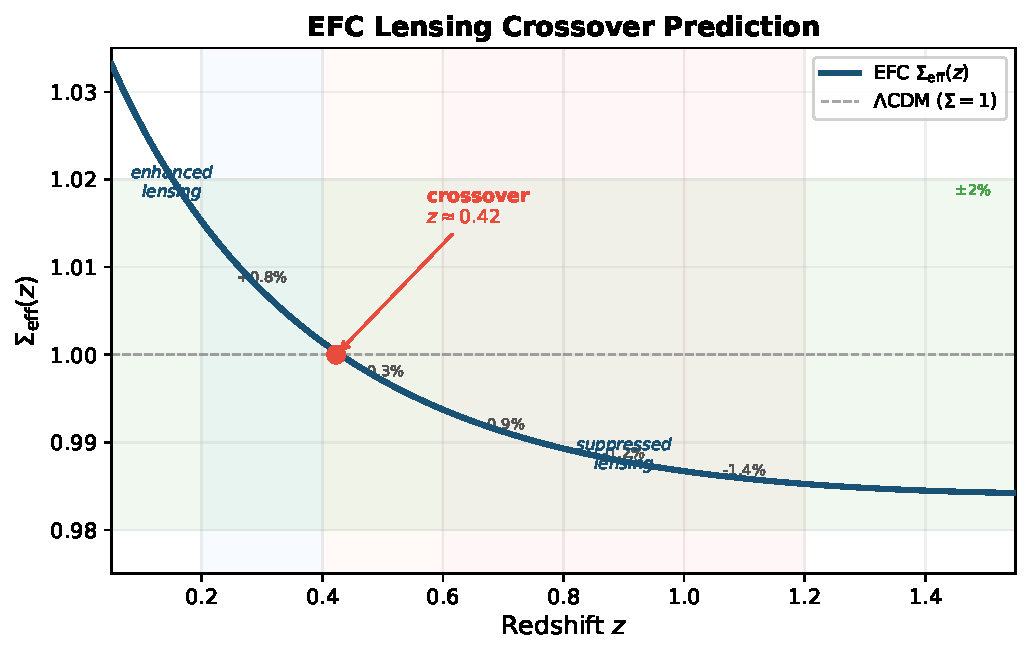
\includegraphics[width=0.85\textwidth]{sigma_eff_crossover.pdf}
\caption{EFC lensing crossover prediction.  The $k$-integrated
effective lensing coupling $\Sigma_{\mathrm{eff}}(z)$ crosses unity at
$z \approx 0.44$, with enhanced lensing ($+2.6\%$) at low redshift and
suppressed lensing ($-1.5\%$) at high redshift.  Shaded bands indicate
Euclid~DR1 tomographic bins.  The green band marks the $\pm2\%$
sensitivity floor.}
\label{fig:crossover}
\end{figure}

% ══════════════════════════════════════════════════════════
\newpage
\section{Variant H MCMC (Negative Result)}

We test the data-driven entropy-gradient growth model
(EFC Variant~H) with two free parameters:
\begin{equation}
\mu(z) = 1 + \bar{S}_0\,\frac{\chi(z)^2}{\chi(z)^2 + \beta_0^2},
\end{equation}
where $\chi(z) = |d\hat{S}/dz|$ from locked Axiom~0 sources, and
$\bar{S}_0$, $\beta_0$ are free MCMC parameters.  Background is
pure \lcdm{} ($\alpha = 0$), compatible with DESI DR2 by construction.

Joint fit to BAO (DESI DR2, 13 points) + $f\sigma_8$ (7 points, with
BOSS DR12 covariance) + $H(z)$ (9 points) + SN\,Ia (Pantheon, 40 bins):

\begin{center}
\begin{tabular}{@{}lcc@{}}
\toprule
Parameter & Value & Interpretation \\
\midrule
$\bar{S}_0$       & $0.210 \pm 0.141$ & $1.49\sigma$ from 0 \\
$\beta_0$          & $2.98 \pm 1.30$   & Poorly constrained \\
$\Delta\mathrm{AIC}$ & $+4.05$ & \lcdm{} preferred \\
$\Delta\mathrm{BIC}$ & $+3.94$ & \lcdm{} preferred \\
$\Delta\log L_{\mathrm{growth}}$ & $-0.014$ & Negligible \\
$\sigma_8$ shift   & $-0.012$ & 1.2\% suppression \\
\bottomrule
\end{tabular}
\end{center}

\textbf{Result~4 (negative).}
\emph{Current data show no preference for the entropy-gradient growth
mechanism.  $\bar{S}_0$ is consistent with zero at $1.5\sigma$.
The two extra parameters are not justified ($\Delta\mathrm{AIC} = +4$).}

This does not falsify EFC (the signal may be below current sensitivity)
but establishes a quantitative baseline for future measurements.

% ══════════════════════════════════════════════════════════
\newpage
\section{Discussion}

\subsection{What has been established}

\begin{enumerate}
\item The EFC action produces a perturbation-sector mechanism
  ($\mu < 1$, $\Sigma > 1$) that is \emph{structurally distinct}
  from standard Horndeski.
\item The mechanism requires the potential gradient $V'(\phi)$ to
  break an exact cancellation between constraint slip and kinetic
  backreaction.
\item The observable signature is a redshift-dependent lensing
  crossover at $z \approx 0.4$--$0.5$ with percent-level amplitude.
\item Growth-sector data currently do not require this extension.
\end{enumerate}

\subsection{Falsification conditions}

\begin{center}
\begin{tabular}{@{}clp{6cm}@{}}
\toprule
ID & Condition & Consequence \\
\midrule
FA4 & $\eta = 1$ at ${>}3\sigma$ & Slip sector falsified \\
FA5 & No viable $(\mu,\Sigma)$ region & Action revised \\
FA-new & $\Sigma_{\mathrm{eff}}(z)$ monotonic & Crossover falsified \\
\bottomrule
\end{tabular}
\end{center}

\subsection{Limitations}

\begin{itemize}
\item The QS approximation breaks down at $k \lesssim 0.03\,h\,\mathrm{Mpc}^{-1}$.
  Full time-dependent perturbation theory is needed for super-horizon modes.
\item The precise crossover redshift depends on the balance between
  $V'$ and the Ricci backreaction, which requires solving the full
  background field equations (Eq.~12--13 of~\cite{magnusson2026action}).
\item Ghost analysis covers only the sub-horizon regime; a full ADM
  Hamiltonian analysis for super-horizon modes remains open.
\end{itemize}

% ══════════════════════════════════════════════════════════
\newpage
\section{Reproducibility}

All results can be reproduced from the following scripts in the
\texttt{AGI-Test} repository:

\begin{center}
\begin{tabular}{@{}lp{9cm}@{}}
\toprule
Script & Purpose \\
\midrule
\texttt{horndeski\_consistency.py} & Horndeski no-go (Sec.~2) \\
\texttt{efc\_perturbation\_engine.py} & Full $(\mu,\Sigma,\eta)$ engine (Sec.~3--4) \\
\texttt{lensing.py} & Lensing engine + kill tests (Sec.~5) \\
\texttt{valley\_robustness\_test.py} & Robustness Monte Carlo (Sec.~4) \\
\texttt{research\_mcmc.py} & Variant~H MCMC (Sec.~6) \\
\texttt{growth\_module.py} & BOSS DR12 $f\sigma_8$ covariance \\
\bottomrule
\end{tabular}
\end{center}

MCMC parameters: 32 walkers, 2000 steps, 800 burn-in, seed\,=\,42.
Data: DESI DR2 BAO (arXiv:2503.14738), BOSS DR12 $f\sigma_8$
(Alam et al.\ 2017), Pantheon SN\,Ia, cosmic chronometers.

% ══════════════════════════════════════════════════════════
\begin{thebibliography}{9}

\bibitem{magnusson2026action}
M.~Magnusson,
\emph{EFC Relativistic Action: Field Equations, Perturbation Theory,
and Extraction of $\mu$, $\Sigma$, $\eta$},
March 2026,
\href{https://doi.org/10.6084/m9.figshare.31876324}{DOI:10.6084/m9.figshare.31876324}.

\bibitem{desi2025}
DESI Collaboration,
\emph{DESI DR2 BAO measurements},
Phys.\ Rev.\ D \textbf{112}, 083515 (2025),
\href{https://arxiv.org/abs/2503.14738}{arXiv:2503.14738}.

\bibitem{pogosian2016}
L.~Pogosian and A.~Silvestri,
\emph{What can cosmology tell us about gravity?},
Phys.\ Rev.\ D \textbf{94}, 104014 (2016).

\bibitem{bellini2014}
E.~Bellini and I.~Sawicki,
\emph{Maximal freedom at minimum cost},
JCAP \textbf{07}, 050 (2014).

\bibitem{alam2017}
S.~Alam et al.\ (BOSS),
\emph{The clustering of galaxies in the completed SDSS-III BOSS},
MNRAS \textbf{470}, 2617 (2017).

\end{thebibliography}

\end{document}
